\documentclass{beamer}
\usetheme{Boadilla}
\usecolortheme{dolphin}
\usefonttheme{serif}
\setbeamertemplate{navigation symbols}{}
\setbeamertemplate{caption}[numbered]
\usepackage{graphicx}
\usepackage{amsmath}
\usepackage{hyperref}
\usepackage{booktabs}
\usepackage{multicol}
\usepackage{pgfplots}
\pgfplotsset{compat=1.18}

\title{An Economic Analysis of Optimal Investment Strategies for Accumulating Housing Down Payments}
\author{Frank Paul Longo II}
\date{\today}

\begin{document}

\begin{frame}
    \titlepage
\end{frame}

\begin{frame}{Overview}
    \tableofcontents
\end{frame}

\section{Introduction}
\begin{frame}{Introduction}
    \begin{block}{Objective}
        Develop optimal investment strategies for first-time homebuyers to save for down payments.
    \end{block}
    \begin{block}{Research Question}
        What are the most effective strategies for different age groups to save for down payments over 5, 10, and 15 years?
    \end{block}
    \begin{block}{Motivation}
        Address the challenges posed by rising housing costs and assist diverse age groups in accelerating their path to homeownership.
    \end{block}
\end{frame}

\section{Financial Literacy: Essential Concepts}
\begin{frame}{Essential Financial Concepts}
    \begin{block}{Stocks}
        Equity investments representing ownership in a company.
    \end{block}
    \begin{block}{Mutual Funds}
        Investment vehicles that pool money from many investors to purchase a diversified portfolio of stocks, bonds, or other securities.
    \end{block}
    \begin{block}{ETFs (Exchange-Traded Funds)}
        Similar to mutual funds but traded on stock exchanges like individual stocks.
    \end{block}
\end{frame}

\section{Typical First-time Homebuyer Profile}
\begin{frame}{Typical First-time Homebuyer Profile}
    \begin{block}{Demographics}
        \begin{itemize}
            \item \textbf{Average Age:} 35 years (2023)
            \item \textbf{Median Income:} \$95,900 (2023)
        \end{itemize}
    \end{block}
    \begin{block}{Marital Status}
        \begin{itemize}
            \item 59\% Married Couples
            \item 19\% Single Females
            \item 10\% Single Males
            \item 9\% Unmarried Couples
        \end{itemize}
    \end{block}
    \begin{block}{Financials}
        \begin{itemize}
            \item \textbf{Average Home Cost:} \$348,000 (2022)
            \item \textbf{Down Payment Saved:} \$8,220
        \end{itemize}
    \end{block}
\end{frame}

\section{Risk Tolerances and Investment Contributions}
\begin{frame}{Investment Contributions by Age Group}
    \begin{block}{Data Source}
        Bureau of Labor Statistics (BLS), Federal Reserve
    \end{block}
    \begin{block}{Annual Income and Contributions}
        \begin{itemize}
            \item \textbf{20-25 years:} 
            \begin{itemize}
                \item Median income: \$45,000
                \item Annual contribution: 10\% of income
            \end{itemize}
            \item \textbf{25-30 years:} 
            \begin{itemize}
                \item Median income: \$60,000
                \item Annual contribution: 15\% of income
            \end{itemize}
            \item \textbf{30-35 years:} 
            \begin{itemize}
                \item Median income: \$80,000
                \item Annual contribution: 20\% of income
            \end{itemize}
        \end{itemize}
    \end{block}
\end{frame}

\section{Data Import and Preparation}
\begin{frame}{Data Sources}
    \begin{block}{Primary Source}
        \textbf{Yahoo Finance (YFinance)}
        \begin{itemize}
            \item Comprehensive financial data on stocks, mutual funds, and ETFs.
        \end{itemize}
    \end{block}
    \begin{block}{Data Coverage}
        \textbf{Date Range:} 10/24/2012 to present (daily frequency)
    \end{block}
\end{frame}

\begin{frame}{Data Snapshot}
    \begin{figure}
        \centering
        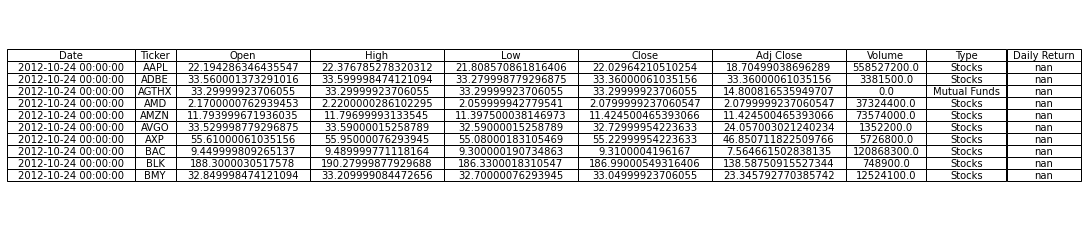
\includegraphics[width=\textwidth]{data_snapshot.png}
    \end{figure}
\end{frame}

\begin{frame}[fragile]{Data Import and Preparation}
    \begin{block}{Loading Data}
        \begin{verbatim}
# import yfinance as yf

# Download data from Yahoo Finance
tickers = ['AAPL', 'MSFT', 'GOOG', 'AMZN',.....]
data = yf.download(tickers, start='2012-10-24', 
end='2024-06-26')
# Save data to CSV
data.to_csv('yfinance_data.csv')
# Load data from CSV
data = pd.read_csv('yfinance_data.csv', index_col='Date')
        \end{verbatim}
    \end{block}
\end{frame}

\section{Exploratory Data Analysis}
\begin{frame}[fragile]{Visualizing Security Count}
    \begin{figure}
        \centering
        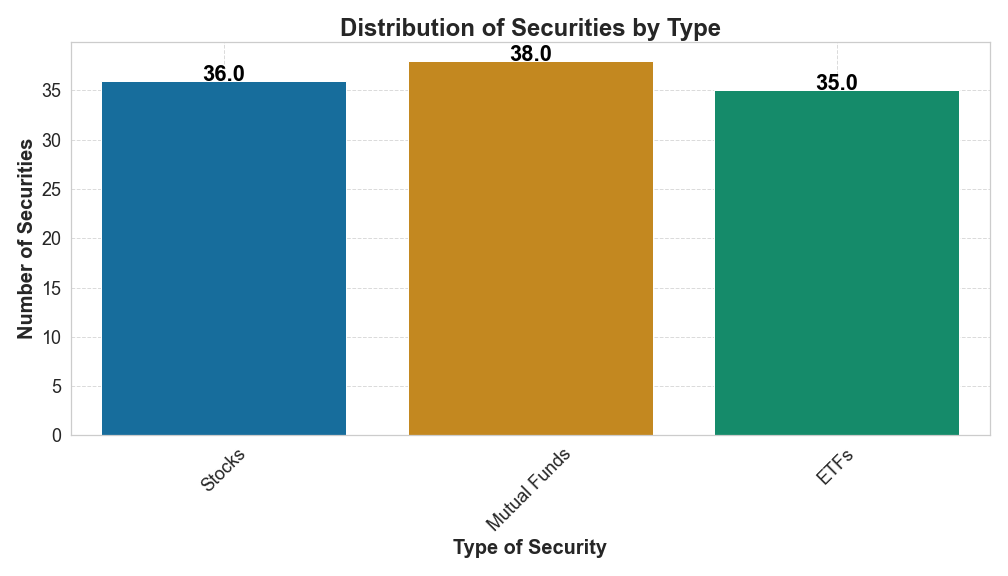
\includegraphics[width=\textwidth]{histogram_security_count.png}
    \end{figure}
\end{frame}

\begin{frame}[fragile]{Visualizing Returns Distribution}
        \begin{figure}
            \centering
            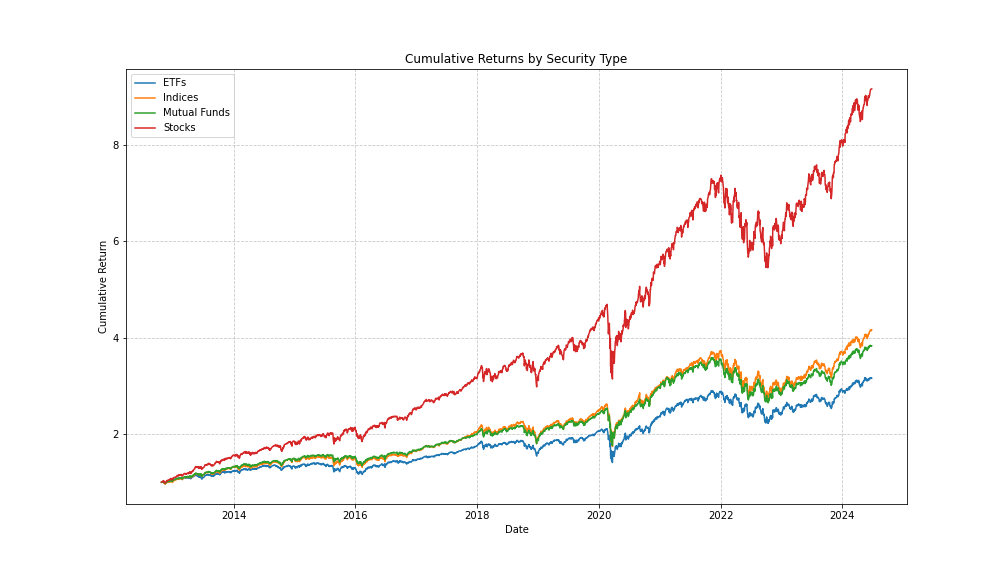
\includegraphics[width=\textwidth]{cumulative_returns_by_type.png}
        \end{figure}
\end{frame}

\section{CAPM and Sharpe Ratio}
\begin{frame}{Capital Asset Pricing Model (CAPM)}
    \begin{block}{Formula} 
        \begin{equation*}
            E(R_i) = R_f + \beta_i (E(R_m) - R_f)
        \end{equation*}
        \footnote{Sharpe, W. F. (1964). Capital asset prices: A theory of market equilibrium under conditions of risk. \textit{The Journal of Finance}, 19(3), 425-442.}
    \end{block}
    \begin{block}{Assumptions}
        \begin{itemize}
            \item Diversified portfolios
            \item Efficient markets
            \item No taxes or transaction costs
            \item Constant risk-free rate
        \end{itemize}
    \end{block}
\end{frame}

\begin{frame}[fragile]{Calculating Beta}
    \begin{block}{Market Return Calculation}
        \begin{verbatim}
# Market return (e.g., S&P 500)
market = yf.download('^GSPC', start='2012-10-24', 
end='2024-09-26')
market_returns = market['Adj Close'].pct_change().dropna()

# Calculate beta for each stock
beta = {}
for ticker in tickers:
    cov_matrix = np.cov(returns[ticker], market_returns)
    beta[ticker] = cov_matrix[0, 1] / cov_matrix[1, 1]
        \end{verbatim}
    \end{block}
\end{frame}

\begin{frame}[fragile]{Calculating Expected Return using CAPM}
    \begin{block}{Expected Return Calculation}
        \begin{verbatim}
# Assuming a risk-free rate of 3% and market return of 8%
risk_free_rate = 0.03
market_return = 0.08

# Calculate expected return for each stock
capm_returns = {}
for ticker in tickers:
    capm_returns[ticker] = risk_free_rate + beta[ticker] * 
    (market_return - risk-free-rate)
        \end{verbatim}
    \end{block}
\end{frame}

\begin{frame}{Sharpe Ratio}
    \begin{block}{Purpose}
        Measures investment performance adjusted for risk.
    \end{block}
    \begin{block}{Formula}
        \begin{equation*}
            S = \frac{E(R_i) - R_f}{\sigma_i}
        \end{equation*}
    \end{block}
    \begin{block}{Components}
        \begin{itemize}
            \item \(E(R_i)\): Expected return
            \item \(R_f\): Risk-free rate
            \item \(\sigma_i\): Std. deviation of excess return
        \end{itemize}
    \end{block}
\end{frame}

\section{Sharpe Ratio Calculation}
\begin{frame}[fragile]{Calculating the Sharpe Ratio}
    \begin{block}{Formula and Calculation}
        \begin{verbatim}
# Sharpe Ratio Calculation
def sharpe_ratio(expected_return, risk_free_rate, stddev):
    return (expected_return - risk_free_rate) / stddev

# Example Calculation
expected_return = 0.0675  # Example from CAPM
risk_free_rate = 0.03
stddev = 0.1  # Example standard deviation

sharpe = sharpe_ratio(expected_return, risk_free_rate,
stddev)
print(f'Sharpe Ratio: {sharpe}')
        \end{verbatim}
    \end{block}
\end{frame}

\begin{frame}{Security Market Line (SML)}
    \centering
    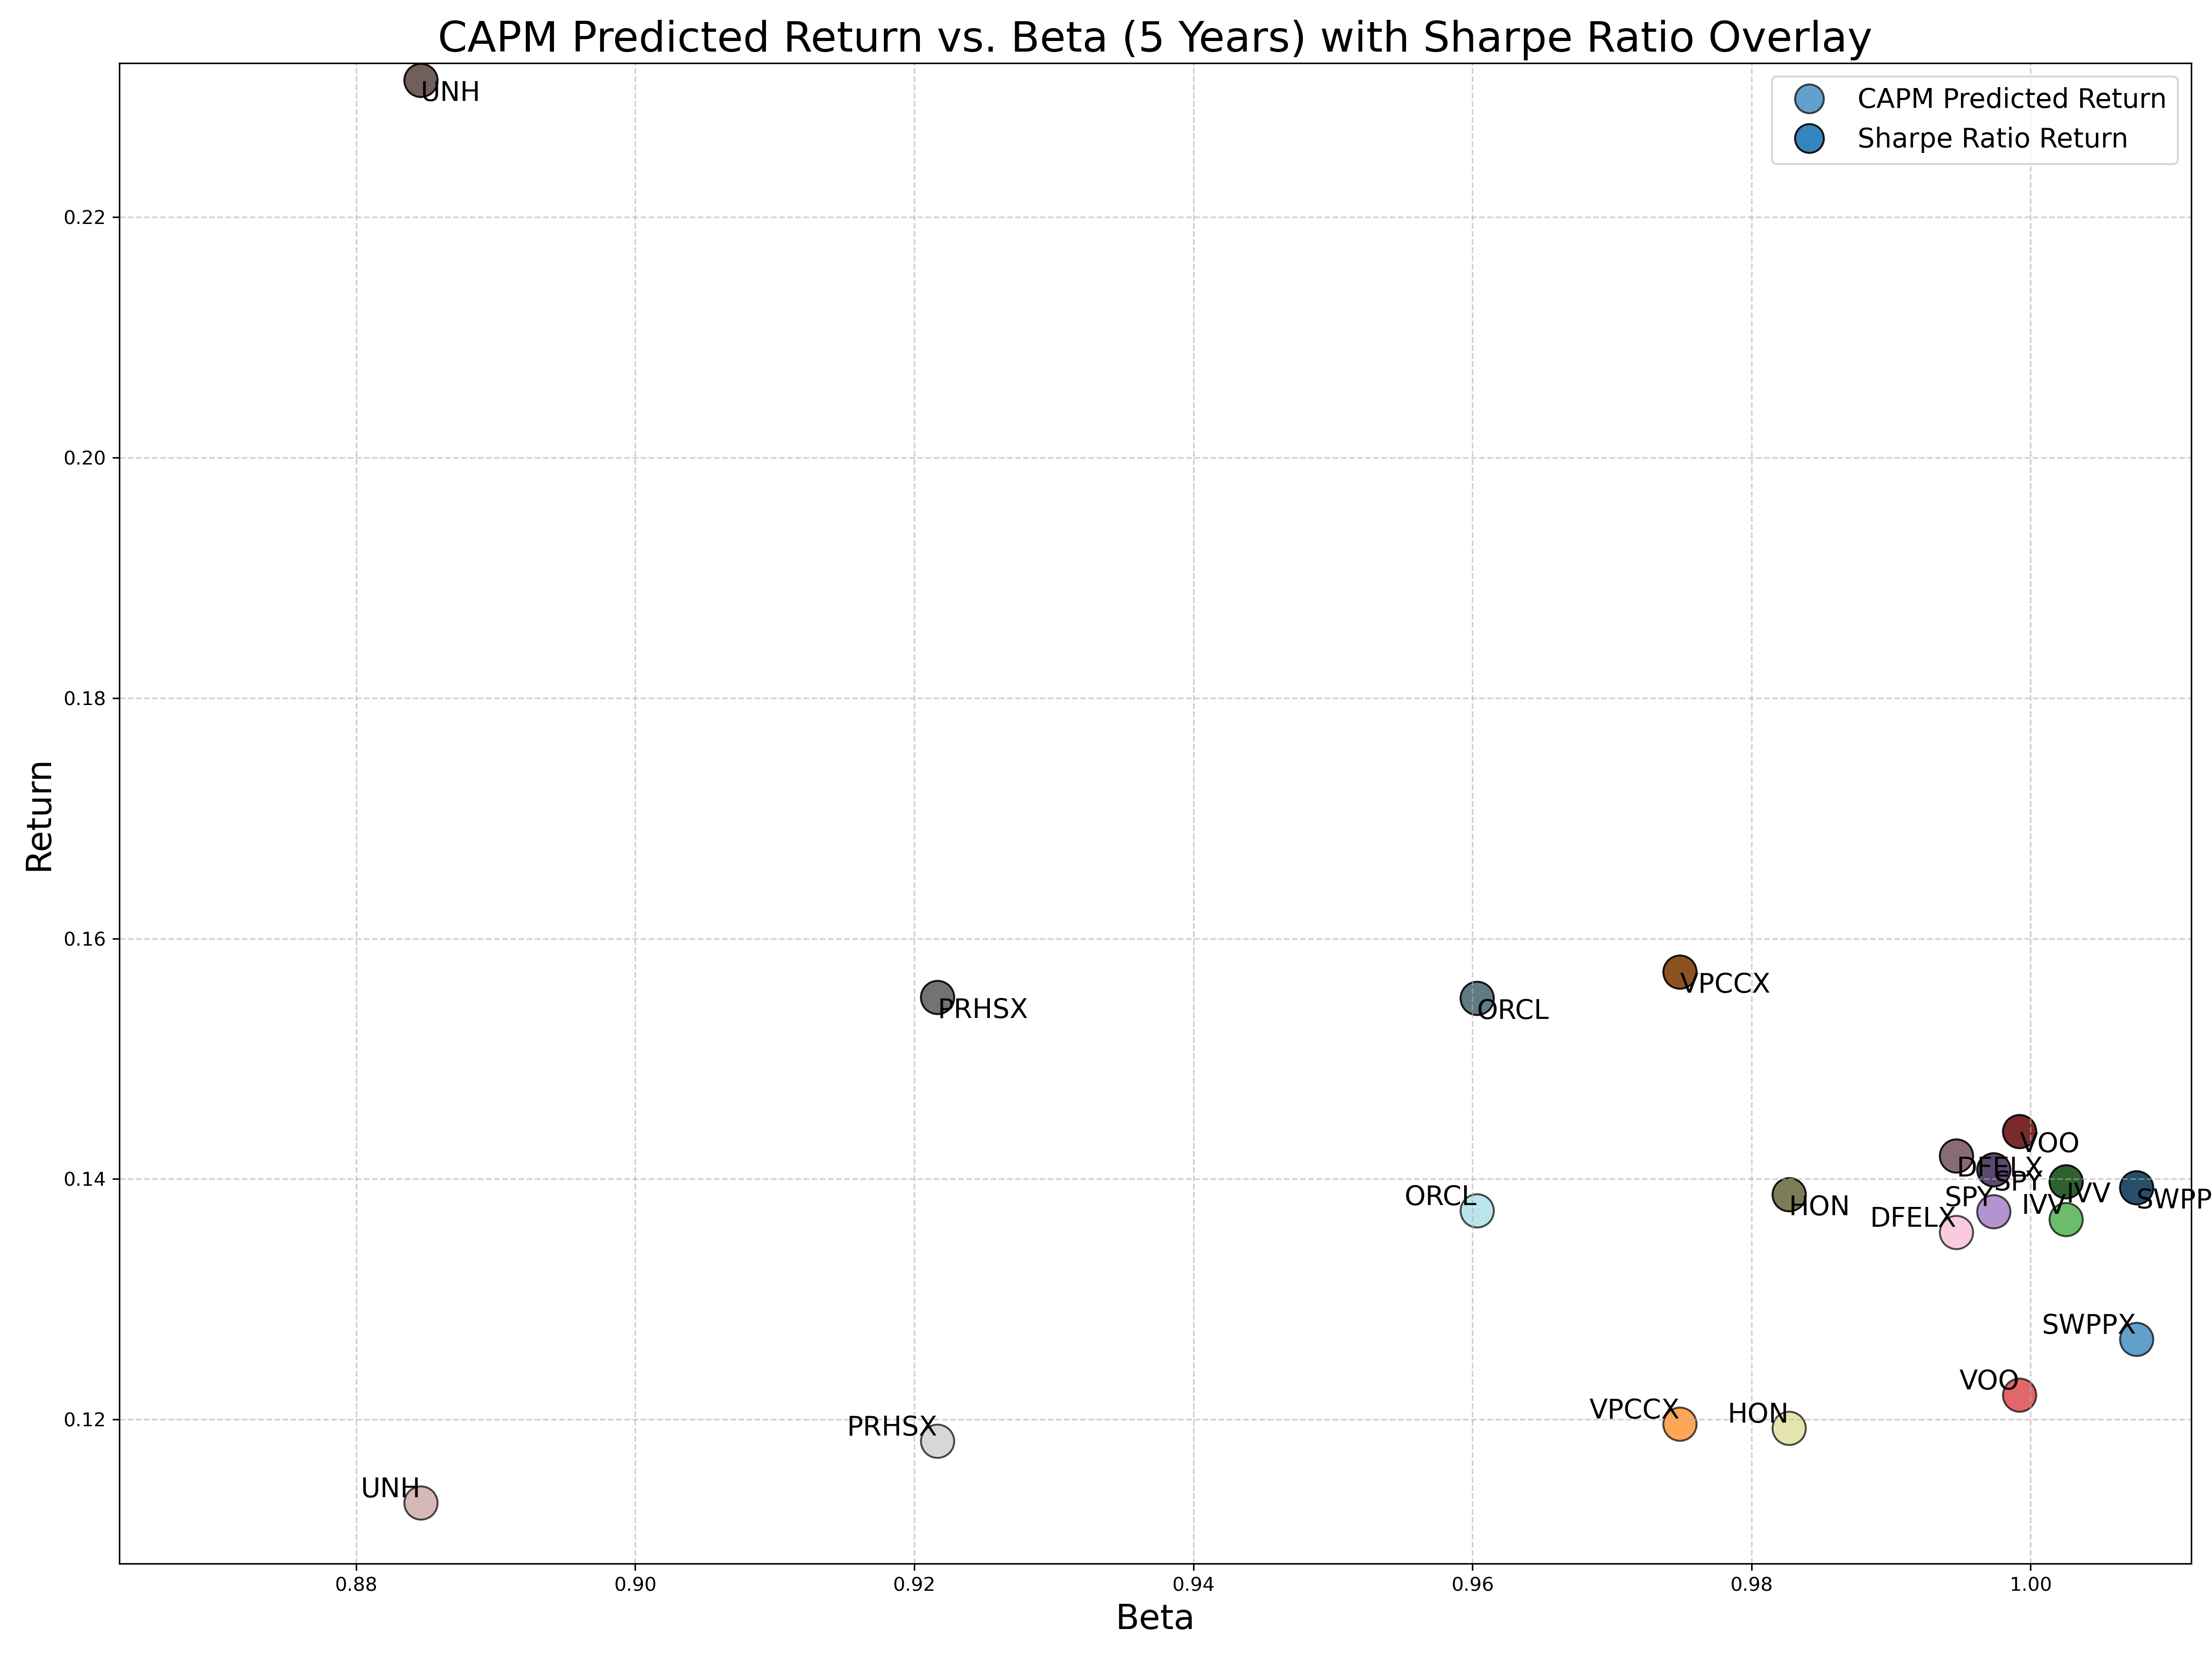
\includegraphics[height=0.8\textheight]{capm_vs_sharpe_5_years.png}
\end{frame}

\begin{frame}{Security Market Line (SML)}
    \centering
    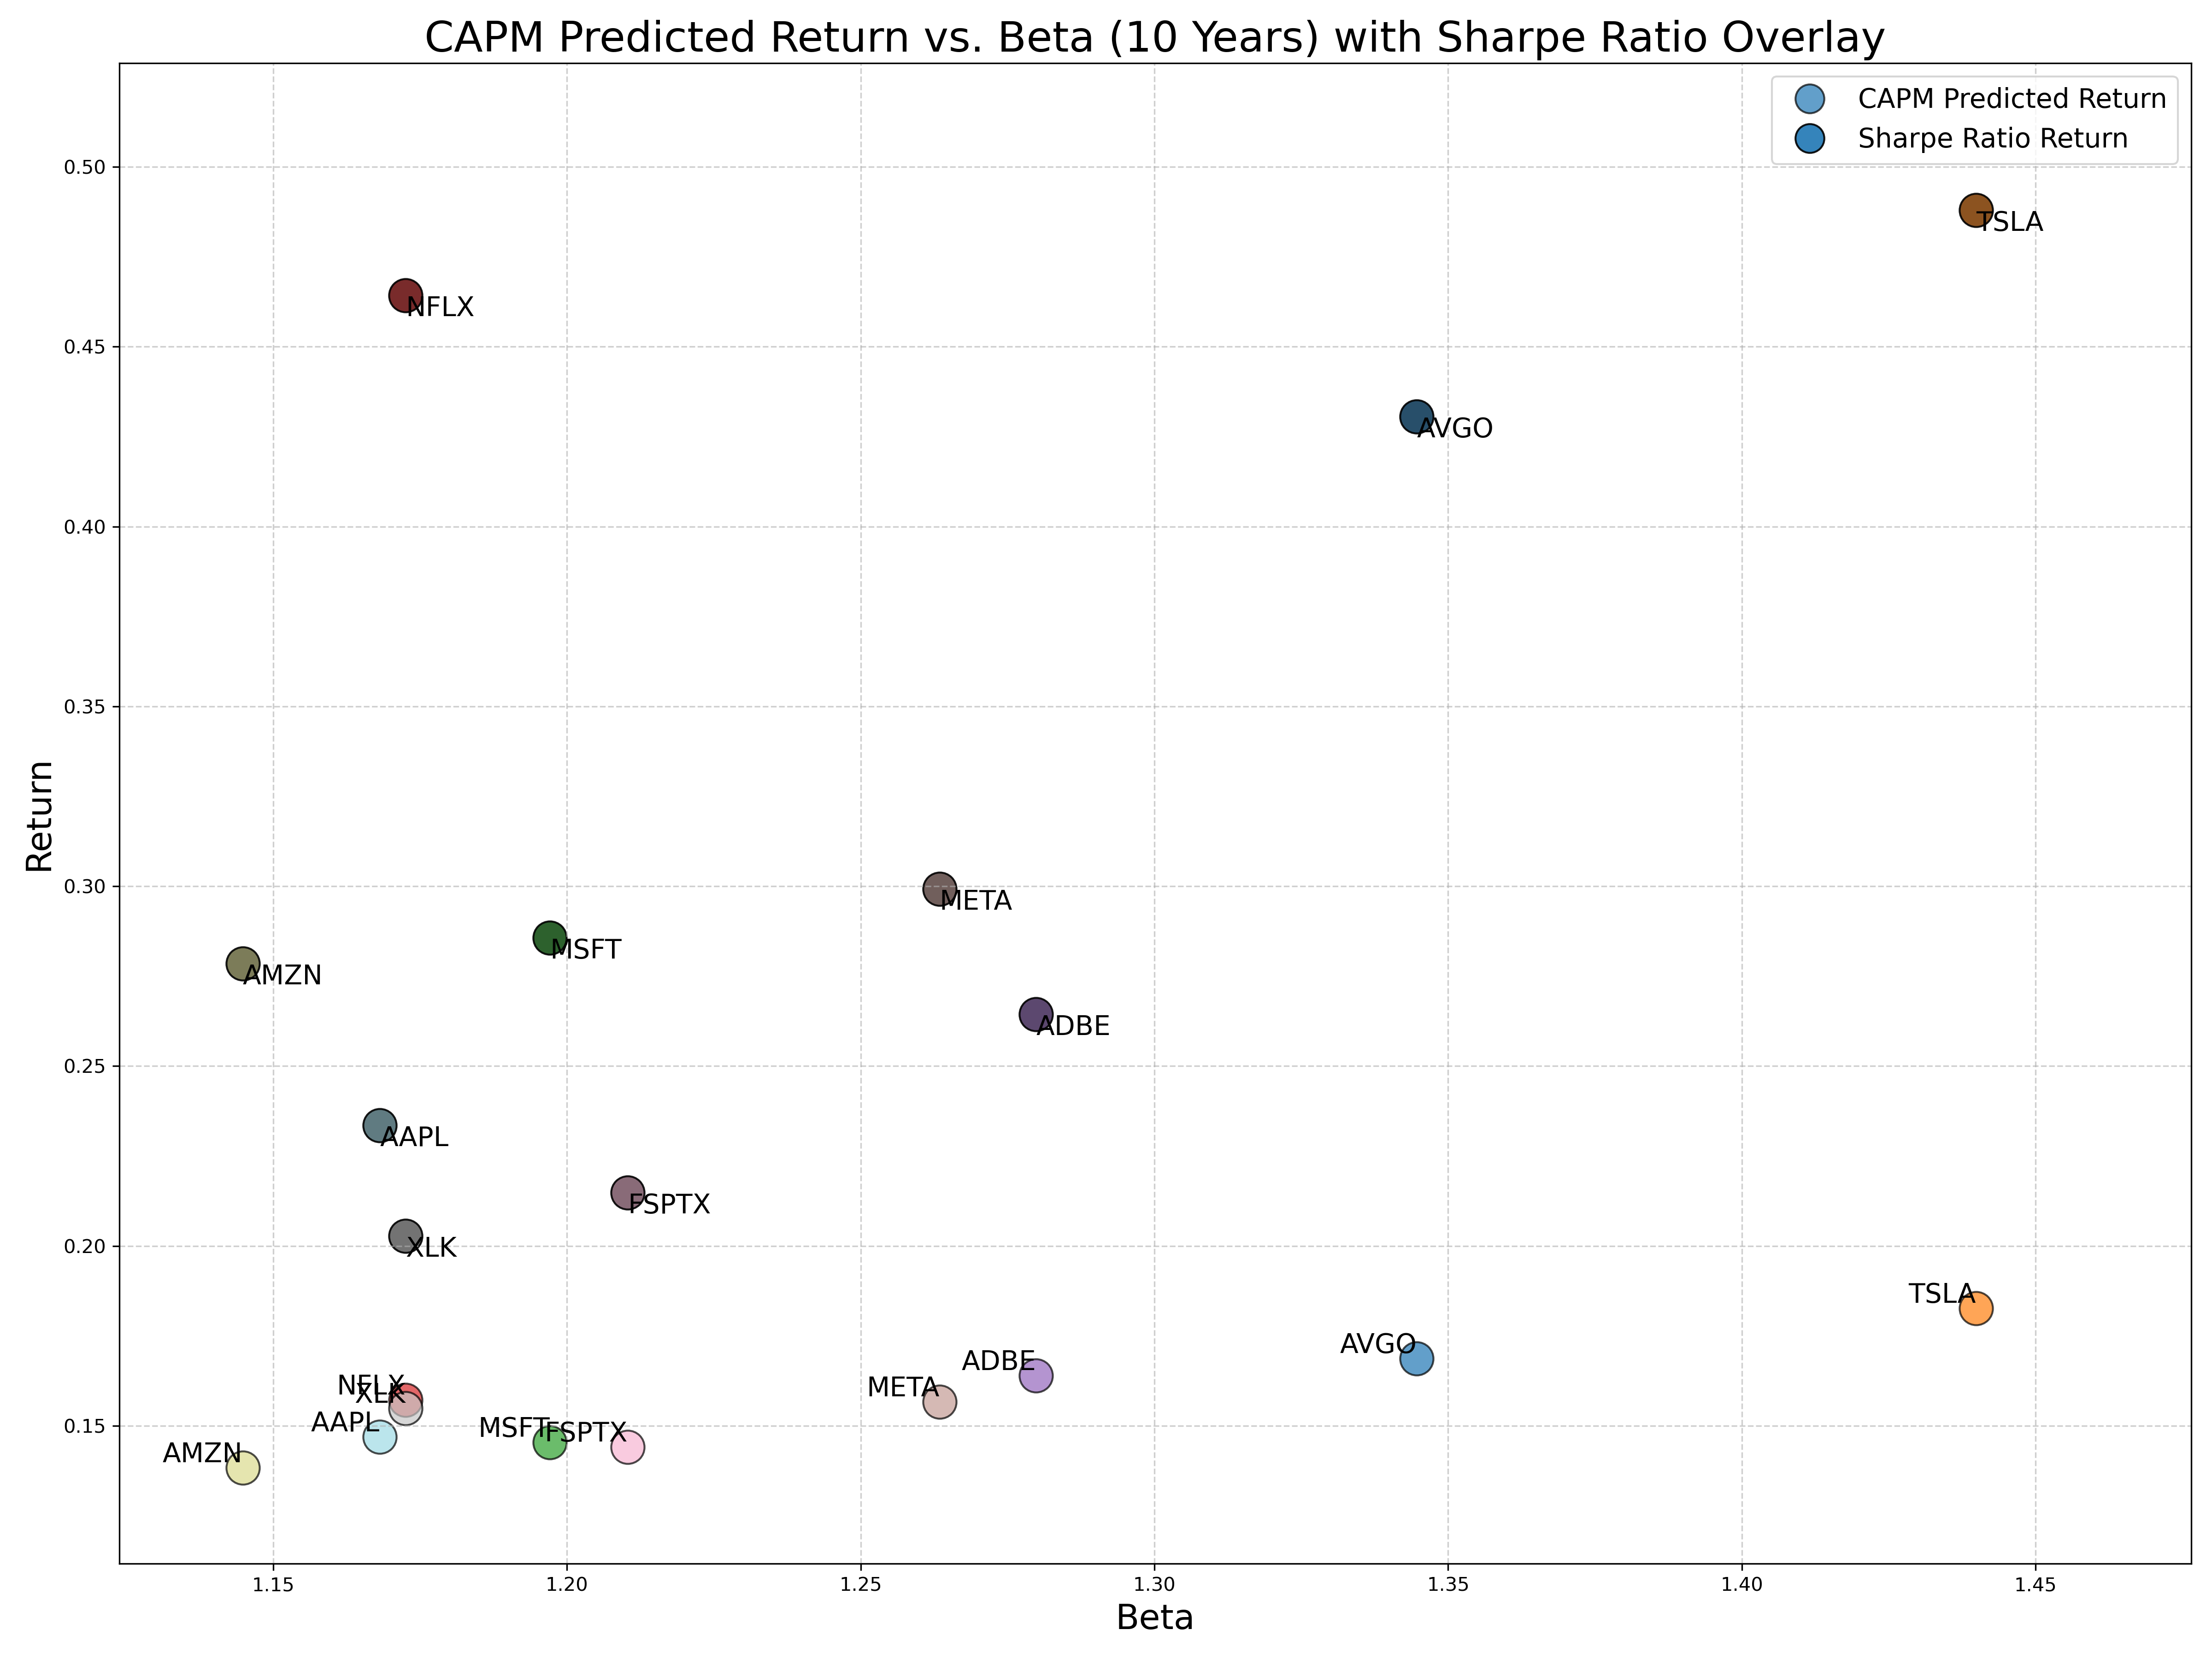
\includegraphics[height=0.8\textheight]{capm_vs_sharpe_10_years.png}
\end{frame}

\begin{frame}{Security Market Line (SML)}
    \centering
    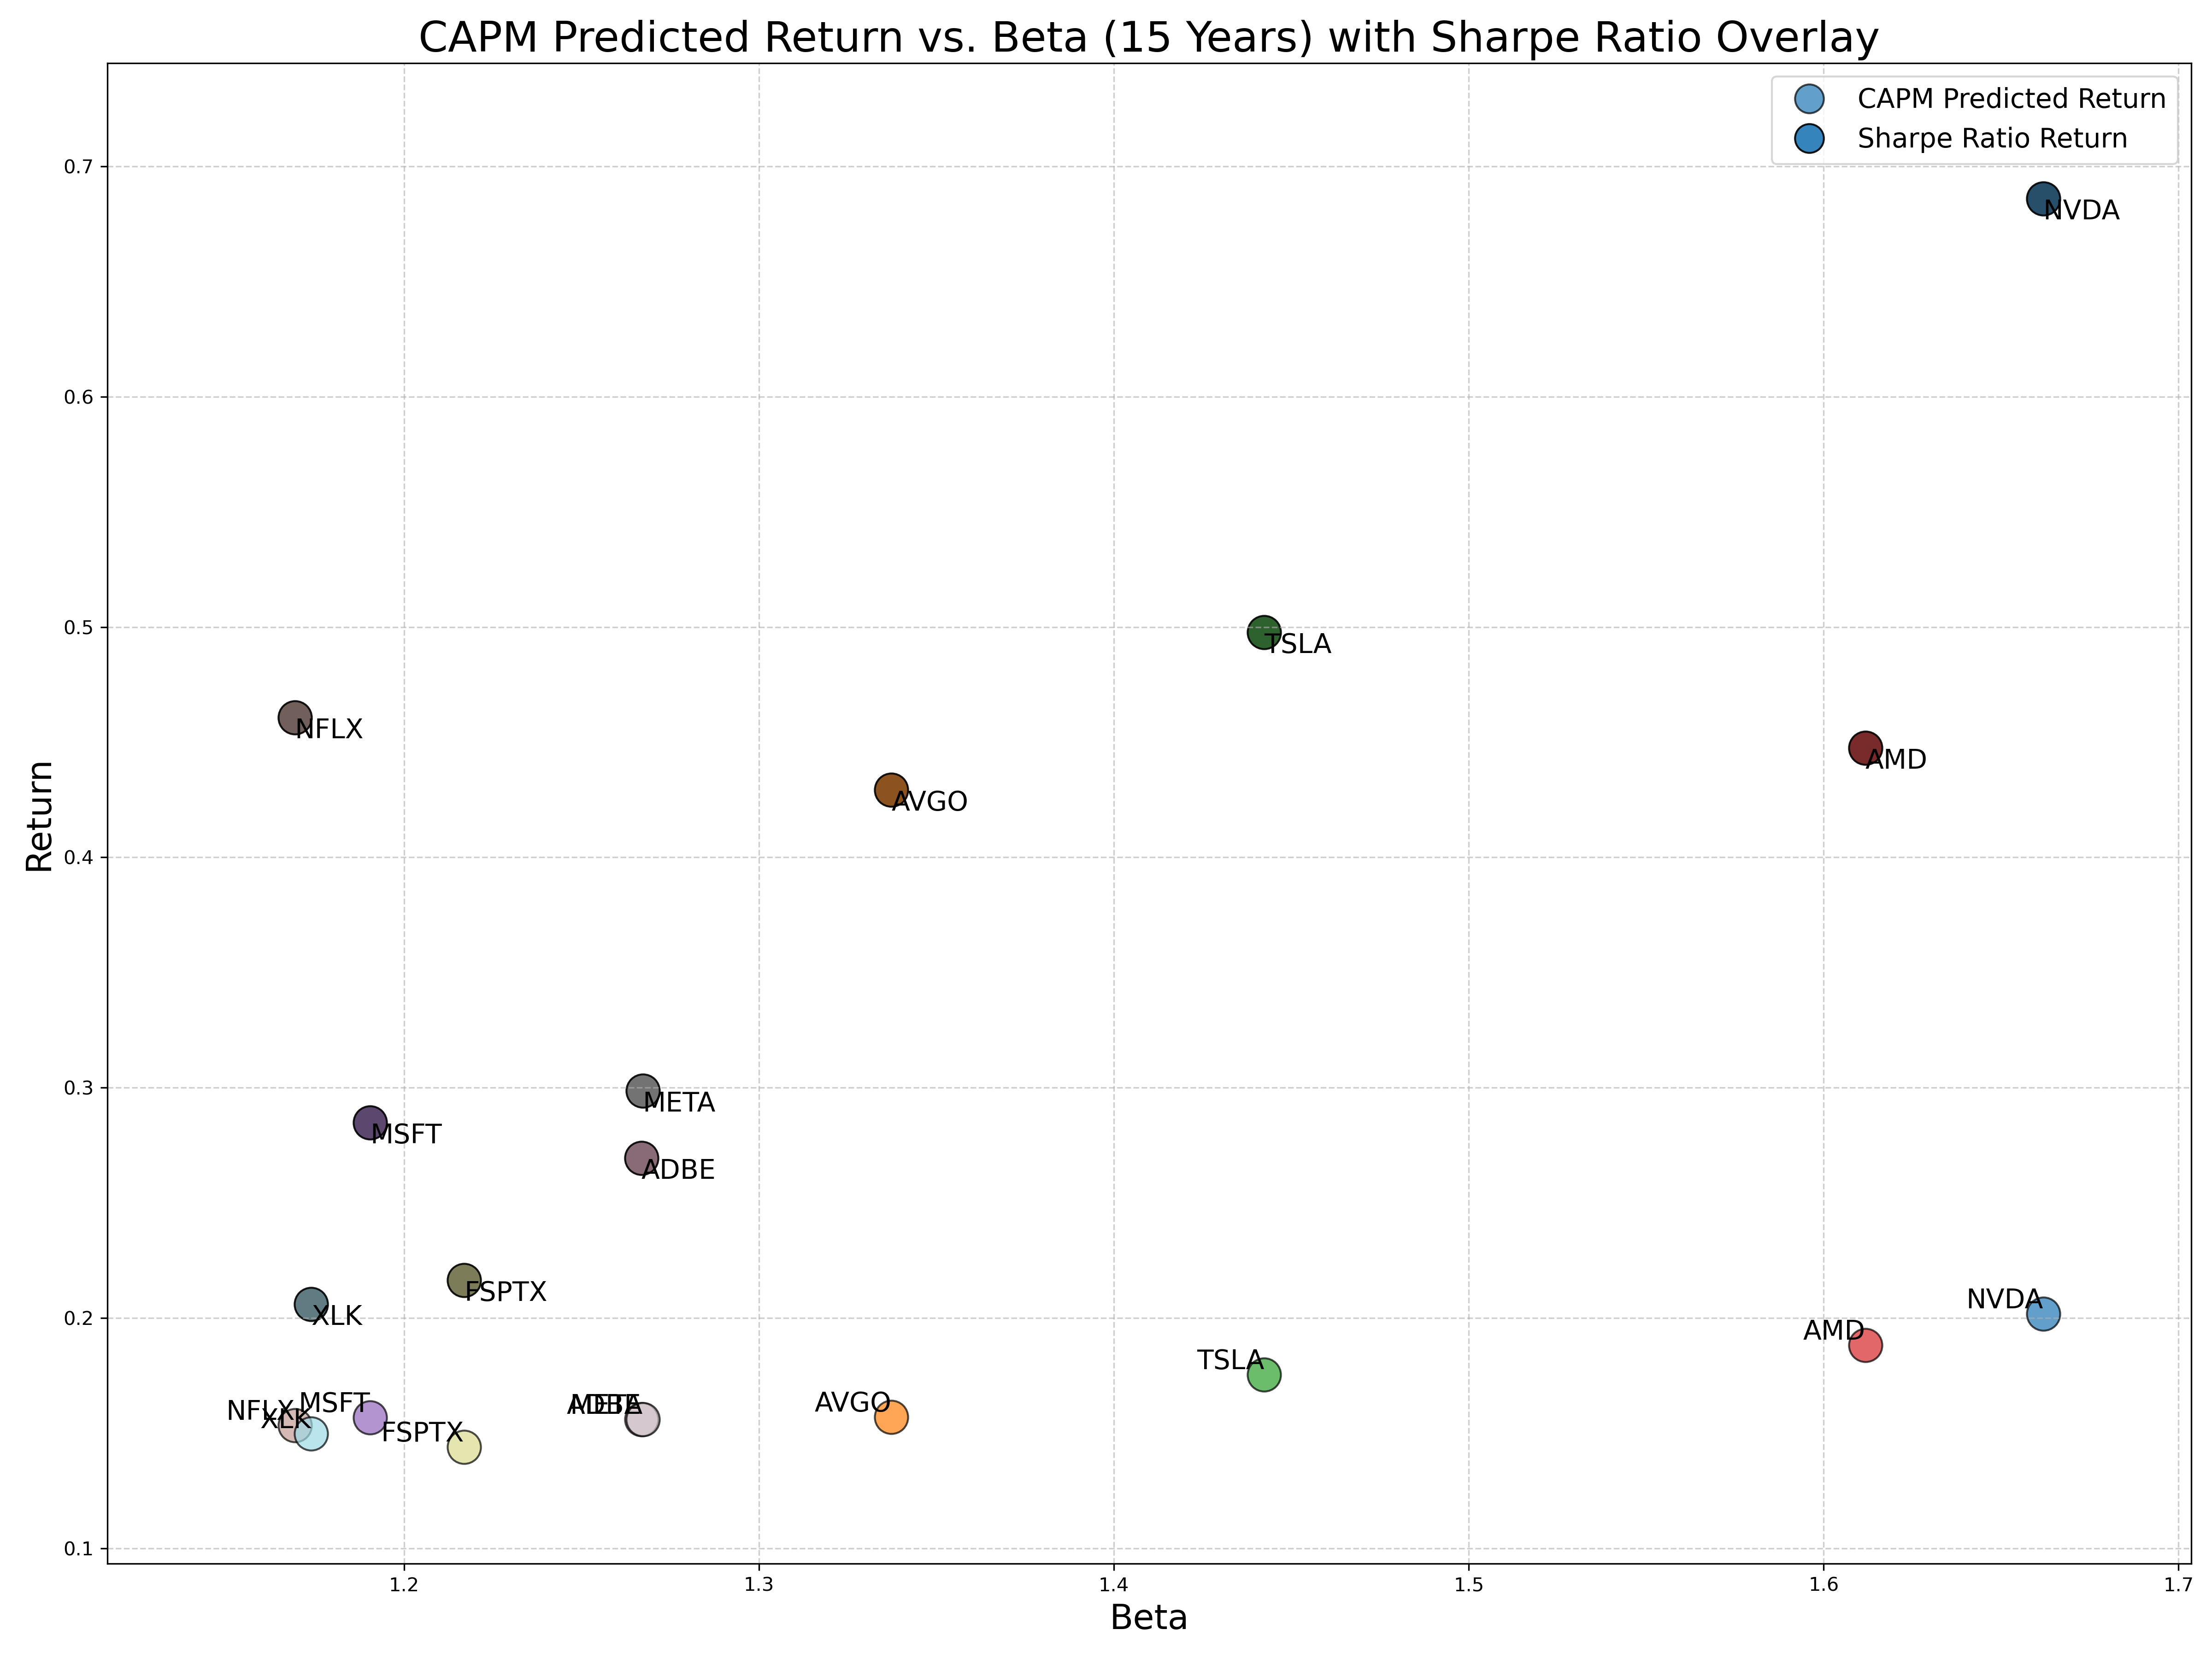
\includegraphics[height=0.8\textheight]{capm_vs_sharpe_15_years.png}
\end{frame}


\section{Modern Portfolio Theory (MPT)}
\begin{frame}{Modern Portfolio Theory (MPT)}
    \begin{block}{Overview}
        Framework for constructing a portfolio to maximize return for a given level of risk.\footnote{Markowitz, H. (1952). Portfolio Selection. \textit{The Journal of Finance}, 7(1), 77-91.}
    \end{block}
    \begin{block}{Formulas}
            \begin{equation*}
                \sigma_p^2 = \sum_{i=1}^{n} \sum_{j=1}^{n} w_i w_j \sigma_{ij}
            \end{equation*}
    \end{block}
    \begin{block}{Definitions}
        \begin{multicols}{2}
            \begin{itemize}
                \item \(E(R_p)\): Portfolio return
                \item \(w_i\): Weight of asset \(i\)
                \item \(E(R_i)\): Return of asset \(i\)
                \item \(\sigma_p^2\): Portfolio variance
                \item \(\sigma_{ij}\): Covariance of assets \(i, j\)
            \end{itemize}
        \end{multicols}
    \end{block}
\end{frame}


\section{Portfolio Optimization}
\begin{frame}{Optimize the Portfolio}
    \begin{block}{Objective}
        Adjust the weights of the assets to maximize the portfolio's expected return for a given level of risk or to minimize risk for a given level of expected return.
    \end{block}
    \begin{block}{Optimization Problem}
        Solve the following optimization problem:
        \begin{equation*}
            \min \sigma_p^2 = \sum_{i=1}^{n} \sum_{j=1}^{n} w_i w_j \sigma_{ij}
        \end{equation*}
        Subject to:
        \begin{equation*}
            \sum_{i=1}^{n} w_i = 1 \quad \text{and} \quad E(R_p) = \sum_{i=1}^{n} w_i E(R_i)
        \end{equation*}
    \end{block}
\end{frame}

\begin{frame}[fragile]{Defining the Optimization Function}
    \begin{block}{Sharpe Ratio Optimization}
        \scriptsize
        \begin{verbatim}
# Define the objective function to minimize
def sharpe_ratio(weights, returns, risk_free_rate=0.03):
    portfolio_return = np.sum(returns.mean() * weights) * 252
    portfolio_stddev = np.sqrt(np.dot(weights.T, 
                                      np.dot(returns.cov() * 252, weights)))
    return - (portfolio_return - risk_free_rate) / portfolio_stddev

# Initial guess for weights
num_assets = len(tickers)
init_guess = num_assets * [1. / num_assets,]

# Constraints and bounds
constraints = ({'type': 'eq', 'fun': lambda weights: np.sum(weights) - 1})
bounds = tuple((0, 1) for asset in range(num_assets))

# Optimize
opt_results = minimize(sharpe_ratio, init_guess, 
                       args=(returns,), method='SLSQP', bounds=bounds, 
                       constraints=constraints)
        \end{verbatim}
    \end{block}
\end{frame}



\begin{frame}{Optimal Portfolio (5 Years)}
    \centering
    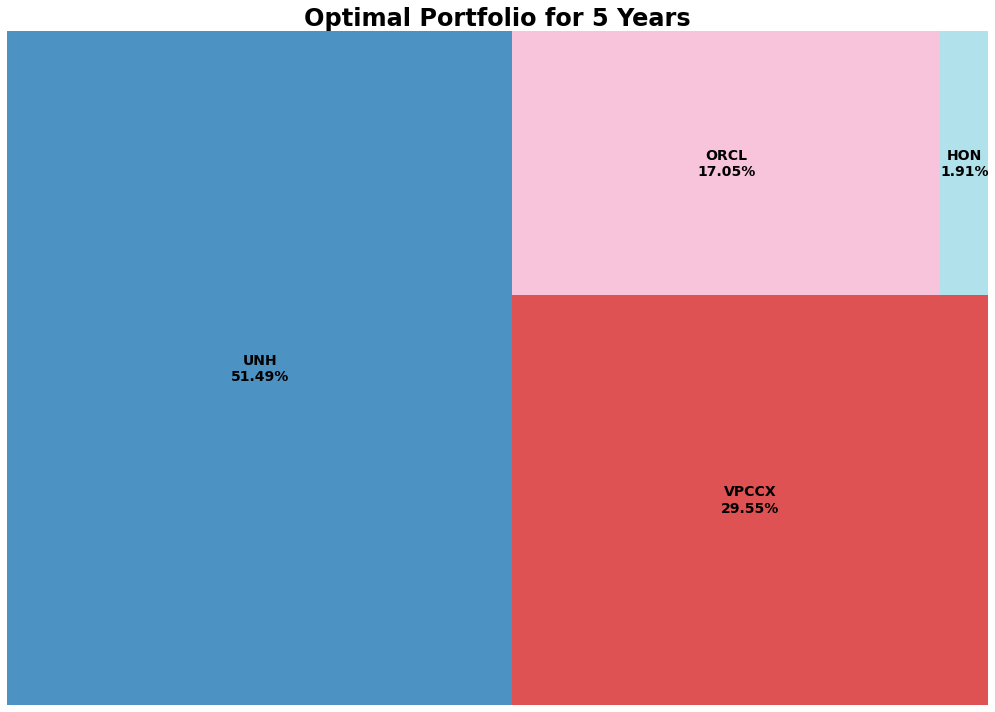
\includegraphics[height=0.8\textheight]{optimal_portfolio_5_years.png}
\end{frame}

\begin{frame}{Optimal Portfolio (10 Years)}
    \centering
    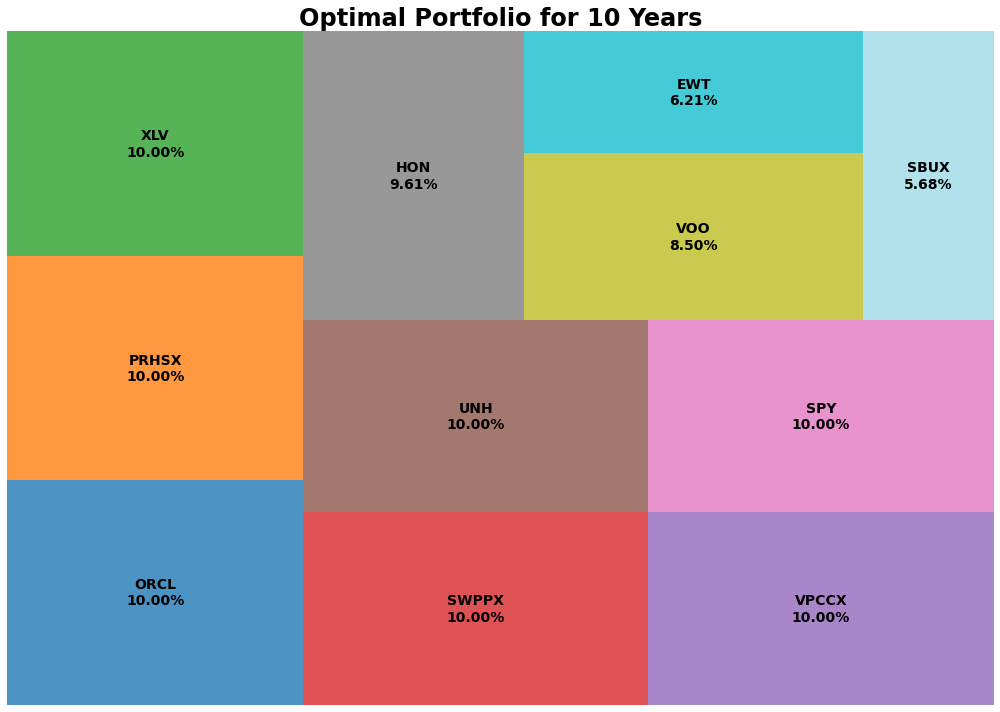
\includegraphics[height=0.8\textheight]{optimal_portfolio_10_years.png}
\end{frame}

\begin{frame}{Optimal Portfolio (15 Years)}
    \centering
    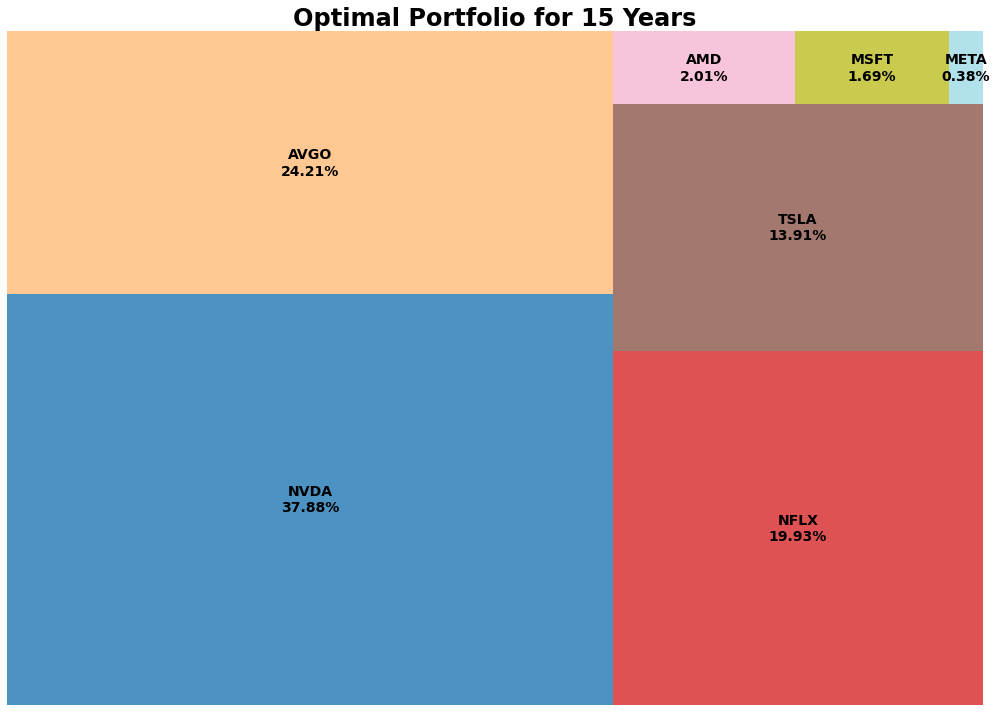
\includegraphics[height=0.8\textheight]{optimal_portfolio_15_years.png}
\end{frame}


\section{Results Interpretation}
\begin{frame}{Results Interpretation}
    \begin{block}{Findings}
        Through this analysis using the Capital Asset Pricing Model (CAPM) alongside the Sharpe Ratio for calculating risk-adjusted return, and Modern Portfolio Theory (MPT), we successfully identified the optimal weights for the selected securities. The analysis revealed that diversification across different asset classes and strategic allocation can significantly enhance the potential for accumulating sufficient down payments over varying time horizons.
    \end{block}
    \begin{block}{Implications}
        These findings underscore the importance of tailored investment strategies for different age groups and income levels. By leveraging these models, first-time homebuyers can make informed decisions that align with their financial goals and risk tolerance.
    \end{block}
\end{frame}

\section{Future Work and Limitations}
\begin{frame}{Future Work and Limitations}
    \begin{block}{Future Work}
        In future research, I plan to incorporate Monte Carlo Simulation to forecast future trends for the optimized portfolio using Modern Portfolio Theory. This will provide a more robust understanding of potential investment outcomes under various market conditions.
    \end{block}
    \begin{block}{Limitations}
        This study's limitations include the assumption of constant risk-free rates and market returns, as well as the exclusion of transaction costs and taxes. Future work should aim to address these limitations to enhance the model's accuracy and applicability.
    \end{block}
\end{frame}

\begin{frame}{Q\&A}
    \begin{block}{Questions and Clarifications}
        Please feel free to ask for any clarifications or additional details regarding the presented research and findings.
    \end{block}
    \vspace{1cm}
    \begin{center}
        \Large \textbf{Thank you for your attention!}
    \end{center}
\end{frame}

\begin{frame}{References (1/2)}
    \begin{block}{}
        \begin{itemize}
            \item Yahoo Finance. (n.d.). Retrieved from \url{https://finance.yahoo.com/}
            \item Robinhood. (n.d.). Retrieved from \url{https://robinhood.com/}
            \item Investment Company Institute. (n.d.). Retrieved from \url{https://www.ici.org/}
        \end{itemize}
    \end{block}
    \begin{block}{}
        \begin{itemize}
            \item Sharpe, W. F. (1966). Mutual Fund Performance. \textit{Journal of Business, 39}(1), 119-138. DOI: 10.1086/294846
            \item Markowitz, H. (1952). Portfolio Selection. \textit{Journal of Finance, 7}(1), 77-91. DOI: 10.2307/2975974
            \item Boyle, P. P. (1977). Options: A Monte Carlo Approach. \textit{Journal of Financial Economics, 4}(3), 323-338. DOI: 10.1016/0304-405X(77)90005-8
        \end{itemize}
    \end{block}
\end{frame}

\begin{frame}{References (2/2)}
    \begin{block}{}
        \begin{itemize}
            \item National Association of Realtors. (2023). 2023 Home Buyer and Seller Generational Trends. Retrieved from \url{https://www.nar.realtor/research-and-statistics/research-reports/home-buyer-and-seller-generational-trends}
            \item Federal Reserve. (2023). Report on the Economic Well-Being of U.S. Households in 2023. Retrieved from \url{https://www.federalreserve.gov/publications/2023-economic-well-being-of-us-households-in-2023.htm}
            \item Bureau of Labor Statistics (BLS). (2023). Income and Expenditures. Retrieved from \url{https://www.bls.gov/income-and-expenditures.htm}
        \end{itemize}
    \end{block}
\end{frame}

\end{document}
